\section{Introduction}

The field of connectomics is concerned with reconstructing the wiring diagram of the brain at nanometer resolutions. 
Recent advancements in image acquisition using multi-beam serial-section electron microscopy (sSEM) has allowed neuroscientists to produce terabytes of electron micrsocopy (EM) image data every hour~\cite{hildebrand2017whole}.
Neuroscientists believe that reconstructing an entire mammalian brain at fine resolution will enable new insights into the workings of the brain~\cite{kasthuri2015saturated}. 
These observations will allow for new advancements in neuromedicine and artificial intelligence. 

Segmenting the image stack into a label volume is a substantial component of this reconstruction process.
In a label volume, every voxel receives a segment label corresponding to a unique neuron. 
Voxels with the same label belong to the same neuron.
It is not feasible for domain experts to manually segment the vast amount of 3-D image data to model an entire brain.
Here we introduce a scalable, top-down segmentation algorithm that also leverages local information.
Partitioning from a top-down approach allows us to apply domain-specific constraints to the segmentation task.

A significant amount of research focuses on automatic reconstruction of the neurons in EM images~\cite{seymour2016rhoananet,nunez2014graph,parag2017anisotropic,zlateski2015image}. %TODO DOUBLE CHECK REFERENCES
All of these algorithms extract neuronal processes through the 3-D volumes using the raw image data as input.
Oftentimes, convolutional neural networks (CNNs) predict membrane probabilities or affinities between voxels and apply simple thresholds to agglomerate the voxels into clusters~\cite{lee2015recursive,ronneberger2015u}.
These \textit{pixel-based} algorithms produce excellent results but currently fall short of complete reconstructions with error rates of approximately $X\%$. %TODO ADD ERROR RATES 
 
\begin{figure*}[h!]
	\centering
	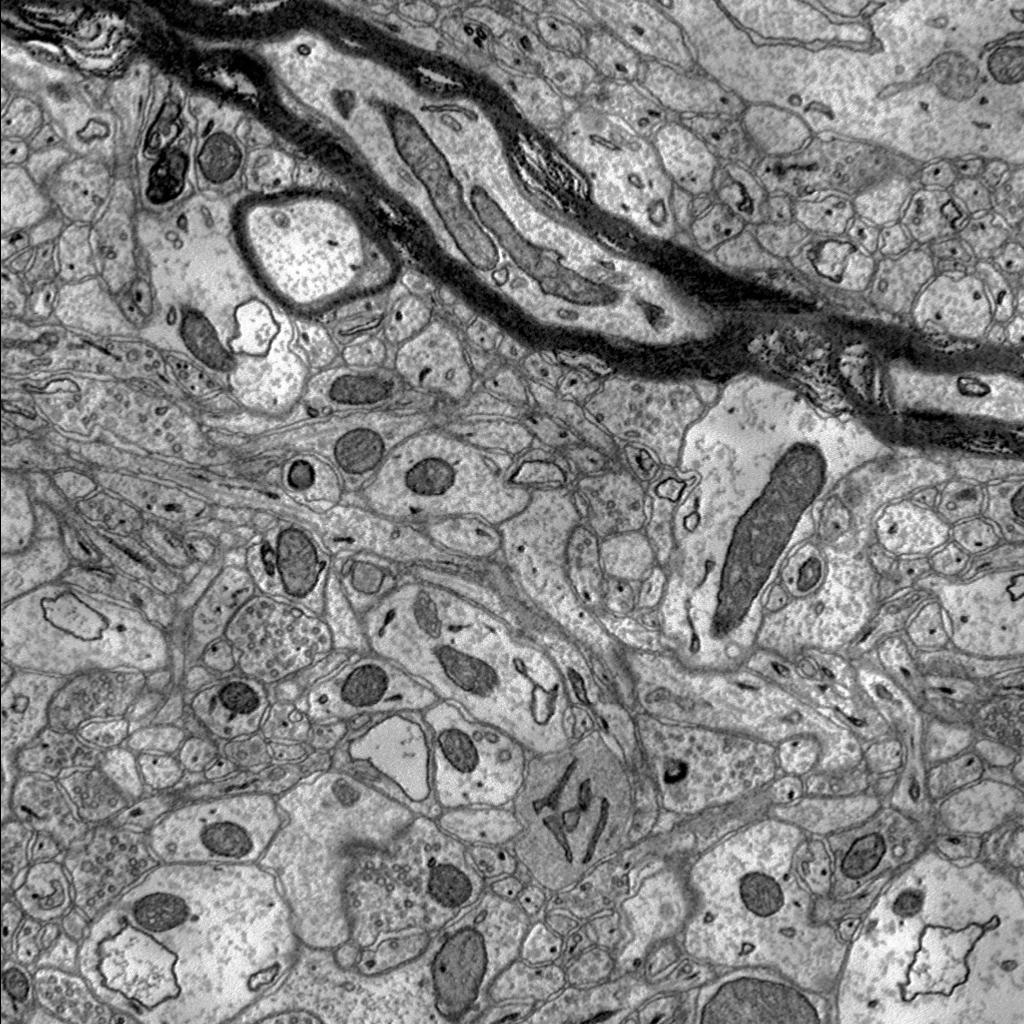
\includegraphics[width=0.22\linewidth]{./figures/pipeline/image.png}
	\hspace{0.025\linewidth}
	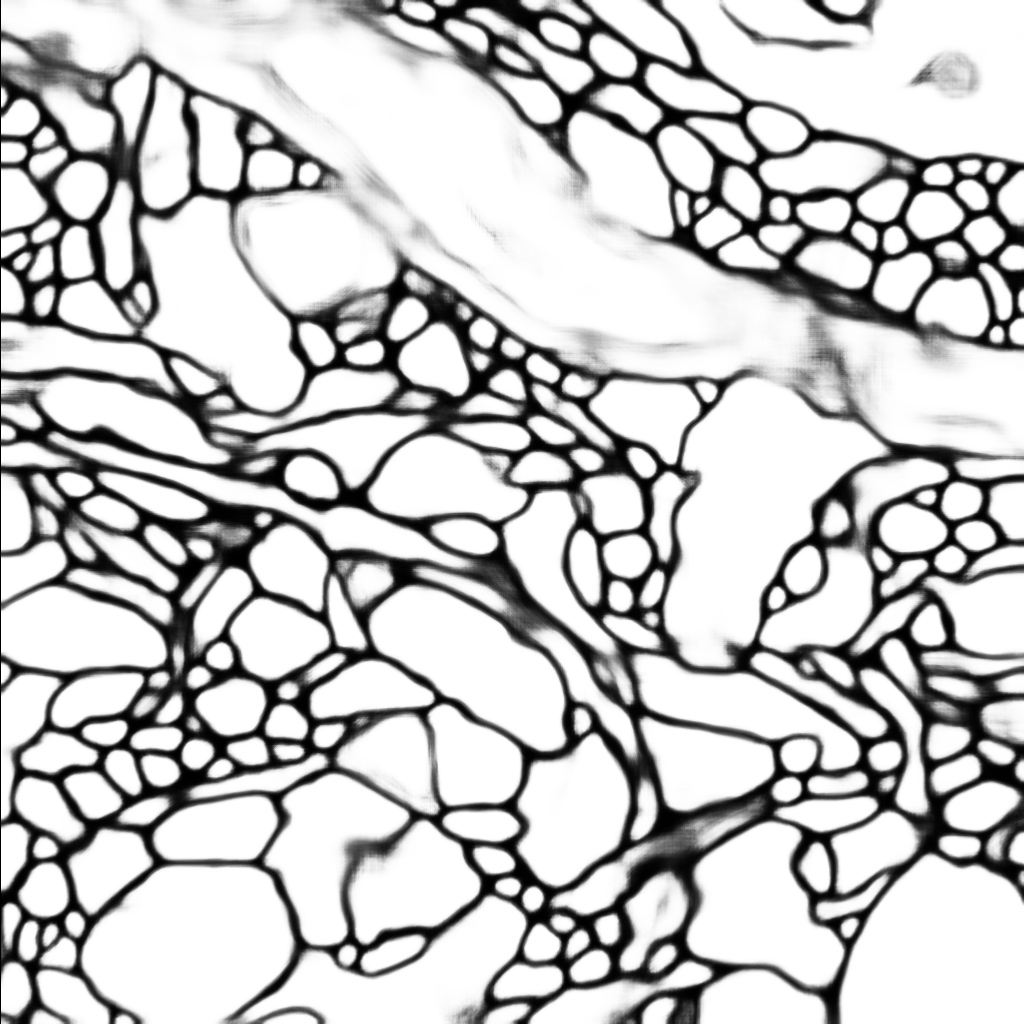
\includegraphics[width=0.22\linewidth]{./figures/pipeline/affinities.png}
	\hspace{0.025\linewidth}
	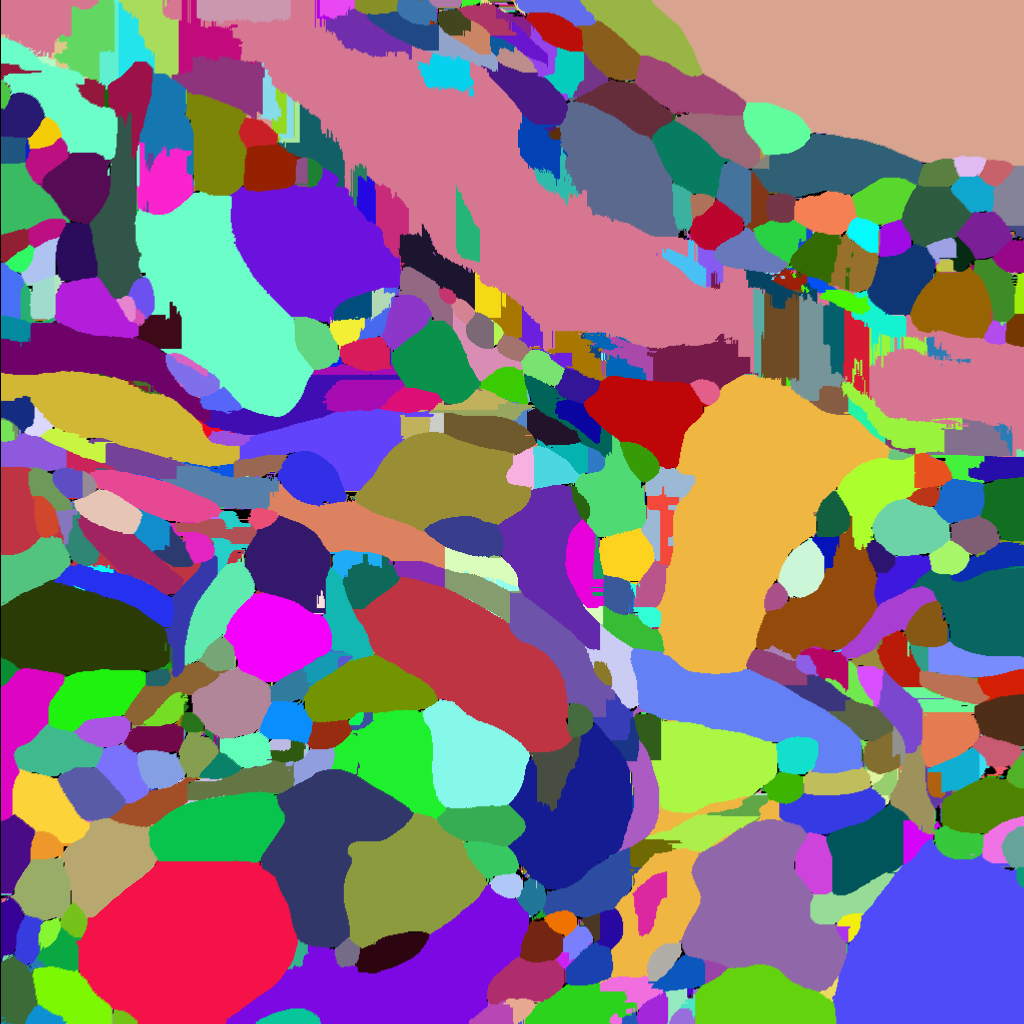
\includegraphics[width=0.22\linewidth]{./figures/pipeline/watershed.png}
	\hspace{0.025\linewidth}
	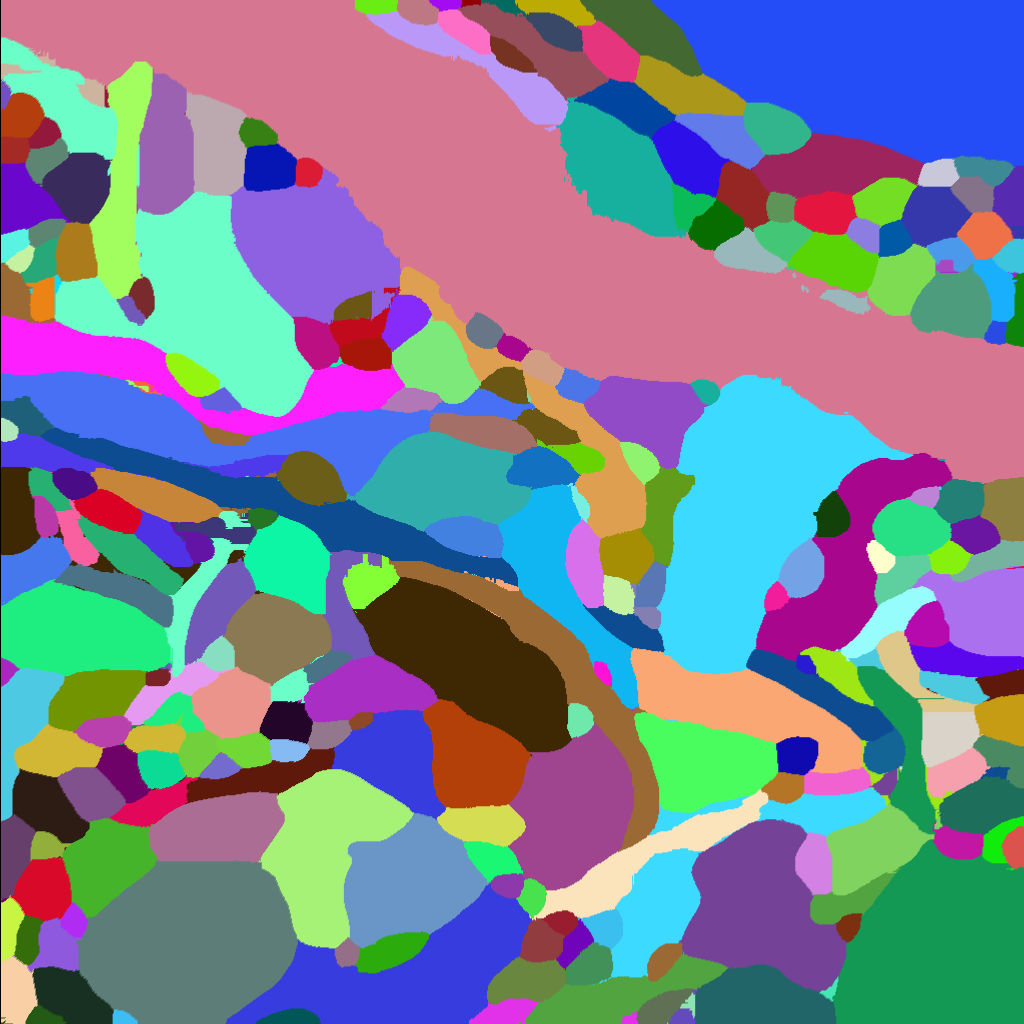
\includegraphics[width=0.22\linewidth]{./figures/pipeline/neuroproof.png}
	\caption{An overview of an existing pipeline in segmentation for connectomics. From left to right: the original EM image data, the output of a CNN predicting voxel affinities, clustering of the affinities using a watershed algorithm, an agglomeration of the supervoxels into larger segments.}
	\label{fig:pipeline}
\end{figure*}

Researchers address the failures of these pixel-based algorithms by training random-forest classifiers to agglomerate an oversegmentation of voxels~\cite{nunez2014graph,10.1371/journal.pone.0125825}.
These classifiers take the output of the pixel-based algorithms as input and generate high-level statistics such as affinity distributions between regions. 
Presently, these methods use hand-designed features despite the evidence that machine-learned features perform better~\cite{bogovic2013learned}. 
These \textit{region-based} algorithms outperform the pixel-based algorithms but do not provide the accuracy needed for large scale reconstructions of the brain.

We present a \textit{segment-based} strategy that builds on the outputs of region-based methods (Figure \ref{fig:teaser}).
We only take as input a segmentation from the region-based agglomeration algorithm. 
This allows us to train on connectomics datasets at a given resolution and image type and test on another resolution.
This is a huge plus considering the sheer amount of expert-hours needed to generate ground truth for these massive datasets.
We extract a graph representation from the input segmentation.
By simplifying the 3-D segments by their skeletons, we can quickly generate the graph nodes and edges. 
We train a 3-D CNN to populate the graph edge weights with bottom-up local information. 
We enforce domain-specific global constraints, such as the underlying biology, using a graph-based partitioning heuristic.
In this we can leverage both local and global information to produce a more accurate segmentation.

Our novel approach creates a level of abstraction over existing region-based agglomeration strategies. 
We take the output of these methods as input and extract a graph structure from that.
This allows us to enforce restrictions on our output that closely follow the underlying biology of these connectomics datasets. 
We use bottom-up information to weight the edges in our graph and top-down information when partitioning the graph. 
This dual approach of assessing local decisions in a global framework produces improvements over the existing region-based methods. 